%  library(knitr); setwd(path <- "c:/seiro/docs/external/seishin/lec_slides/2024/"); system("recycle c:/seiro/docs/external/seishin/lec_slides/2024/MaximisationSlides/cache/"); knit("MaximisationSlides.rnw", "MaximisationSlides.tex"); system("platex MaximisationSlides"); system("pbibtex MaximisationSlides"); system("dvipdfmx MaximisationSlides")

\input{c:/seiro/settings/Rsetting/knitrPreamble/knitr_beamer_preamble169.rnw}
%\input{c:/seiro/settings/Rsetting/knitrPreamble/knitr_beamer_preamble169_ho.rnw}
%\input{c:/seiro/settings/Rsetting/knitrPreamble/knitr_beamer_preamble.rnw}
%\input{c:/seiro/settings/Rsetting/knitrPreamble/knitr_beamer_preamble_ho.rnw}
\definecolor{bondiblue}{rgb}{0.0, 0.58, 0.71}
\definecolor{bondibluelight}{rgb}{0.0, 0.3, 0.41}
\definecolor{aqua}{rgb}{0.0, 1.0, 1.0}
\definecolor{bittersweet}{rgb}{1.0, 0.44, 0.37}
\definecolor{azure}{rgb}{0.0, 0.5, 1.0}
\definecolor{applegreen}{rgb}{0.55, 0.71, 0.0}
\definecolor{darkpastelgreen}{rgb}{0.01, 0.75, 0.24}
%\setbeamercolor{background canvas}{bg=bondibluelight}
\setbeamercolor{background canvas}{bg=darkdarkblue}
\setbeamercolor{normal text}{fg=white}
\setbeamercolor{item}{fg=aqua}
\mode<handout>{\setbeamercolor{item}{fg=blue!70!black}}
\mode<handout>{\setbeamercolor{background canvas}{bg=white}}
\mode<handout>{\setbeamercolor{normal text}{fg=black}}
\hypersetup{
%linkcolor = lightblue, urlcolor = lightblue
linkcolor = blue!50, urlcolor = green!80
, citecolor = blue!50
}
\setbeamercovered{invisible}
\newcommand{\DescPause}{\hspace{-.25em}\phantom{\thebeamerpauses}\pause}

\usepackage{pgfplots}
\pgfplotsset{compat=1.11} % this sets default coordinate system to axis cs in axis environment
\usetikzlibrary{intersections, arrows, calc, positioning, overlay-beamer-styles}

\newcounter{angle}
\setcounter{angle}{0}
\usepackage{centernot}
\usepackage{usebib}

\begin{document}
\setlength{\baselineskip}{12pt}






\title[4]{\large 微分}
\author[Ito]{Seiro Ito}
\institute[IDE, Sacred Heart]{Institute of Developing Economies, Japan}
\date[Fall, 2024]{Fall, 2024\\\vspace{1ex} Department of International Exchange, Sacred Heart University}
\logo{SHU, IDE}


\frame{\titlepage}
\setcounter{page}{1}

%\setbeamercovered{transparent = 40}
%\setbeamercolor{normal text}{fg=turquoiseazure2, bg=}
%\setbeamercolor{alerted text}{fg=black, bg=}
%\usebeamercolor{normal text}
%\setbeamercovered{transparent=0}
\def\Perp{\mkern2mu\rotatebox[origin=c]{90}{$\models$}\mkern2mu}

\begin{frame}[t]{}
微分differentiationとは関数の傾きなどを知る手法です。\\~\\

\pause
傾きを知りたい理由は、関数が最大/最小になる点を知りたいからです。
\begin{itemize}\footnotesize
\vspace{1.0ex}\setlength{\itemsep}{1.0ex}\setlength{\baselineskip}{12pt}
\pause
\item	生涯効用を最大化する子ども期の教育年数は何年か。[効用関数]
\pause
\item	教育の純便益(=便益-費用)関数を最大化する遠隔教育時間は何時間か。[純便益関数]
\pause
\item	企業の利潤を最大化する雇用時間は何時間か。[利潤関数]\\[2ex]
\end{itemize}
\pause
多くの場合、変数を変化させると便益と費用が逆の方向に動くトレードオフがあります。関数は単調に増えたり減ったりする単調関数ではありません。よって、変数の値を適切に選ぶ必要があります。
\begin{dinglist}{43}\footnotesize
\vspace{1.0ex}\setlength{\itemsep}{1.0ex}\setlength{\baselineskip}{12pt}
\pause
\item	教育年数を増やす: 人的資本が増えるが、収入を得る期間が減る。
\pause
\item	遠隔教育時間を増やす: 教室に来られない生徒の人的資本が増えるが、教室に来られる生徒の対面での人的資本蓄積が減る。
\pause
\item	雇用時間を増やす: 収入が増えるが、支払う労働費用も増える。\\[2ex]
\end{dinglist}
\pause
\textcolor{red}{関数が最大化する点は、関数が水平になる点=関数の傾きがゼロになる点}です。
\end{frame}

\begin{frame}[t, label=fx]{}
\onslide<1->{以下は$y=f(x)$という1変数$x$の関数$f(x)$を描いています。\\~\\}
\onslide<3->{関数の微分は$f'(x)$と表記しますが、その意味は\textcolor{red}{$x$での$f(x)$の傾き}のことです。\\~\\}
\onslide<4->{微分とは変数$x$が僅かに変化したときの関数$f$の反応を計算したものだからです。微分してゼロとなる地点とは、傾きがゼロ$f'(x)=0$となる$x$のことを指します。}\\~\\
%\onslide<5->{$f(x)=1+2x\textcolor{azure}{-.25}x^{2}$のような2次関数で\textcolor{azure}{2次の係数が負}の場合は、最大値が1つだけあります。よって、$f'(x)=0$を満たす$x$は関数の最大値を与えます。}

%fx <- function(x) 8+.5*x-.4*x^(2)+(1/30)*x^(3)
%x1 <- c(.68337, fx(.68337)) 0.683370 8.165525
%x2 <- c(7.3166, fx(7.3166))7.316600 3.301142

\setbeamercovered{invisible}
\begin{columns}[T]
\column{.5\paperwidth}
\onslide<2->{
\hfil\mpage{.5\paperwidth}{
\begin{tikzpicture}[ 
axis/.style={very thick, ->, >=stealth'},
dashed line/.style={dashed, thin},
every node/.style={},
background rectangle/.style = {fill = gray90},
]
\begin{axis}[
  scale = .65,
  axis equal image, % forces a square plot
  clip = false, % allows plotting outside axis bounds
  axis x line=center, axis y line=center,
  xlabel = {$x$}, ylabel = {$y$},
  xtick={100}, ytick={100}, % effectively drops axis ticks
  xlabel style={below right}, ylabel style={above left},
  xmin=0, xmax=11,
  ymin=0, ymax=10]
\coordinate (origin) at (axis cs: 0, 0) ;
\path[name path=xaxis, gray] (0, 0) -- (axis cs: 10, 0);
\path[name path=yaxis, gray] (0, 0) -- (axis cs: 0, 10);
\coordinate (m1) at (axis cs: 4, 5) ;
% curves
\addplot [name path=X2curve, no marks, line width = .5pt, domain=0.01:7, smooth] {1+2*x-.25*x^(2)} node[below right] (fend) {\small $f(x)=1+2x-.25x^{2}$};
\addplot [name path=Hor1, azure, no marks, line width = .5pt, domain=0.01:9, dashed, smooth] (0, 5) node [left] {5} -- (axis cs: 9, 5) node[right] (Dend) {\small $f'(x)=0$};
\addplot [name path=Ver1, azure, no marks, line width = .5pt, domain=0.01:9, dashed, smooth] (4, 0) node [below] {4} -- (m1);
% intersections of curves
\fill [azure] (m1) circle (3pt);
% x and y coordinates of intersections
\coordinate (m1Xaxis) at (m1 |- origin) ;
\end{axis}
\end{tikzpicture}
}}
\column{.45\paperwidth}
\vspace{1cm}
微分の定義
\[
f'(x)=\lim_{h\rightarrow 0}\frac{f(x+h)-f(x)}{h}.
\]
\end{columns}

\mpage{\paperwidth}{\onslide<5->{\mpage{.5\paperwidth}{$f'(x) = 2-.5x=0 \quad \Rightarrow \quad x = 4$\\ \hyperlink{DiffFormulae}{\beamergotobutton{微分公式}} $f(x)=bx^{n} \Rightarrow f'(x)=bnx^{n-1}$}}}
\end{frame}

\begin{frame}[t, label=fx]{}
\onslide<1->{以下は$y=f(x)$という1変数$x$の関数$f(x)$を描いています。\\~\\}
\onslide<1->{関数の微分は$f'(x)$と表記しますが、その意味は\textcolor{red}{$x$での$f(x)$の傾き}のことです。\\~\\}
\onslide<1->{微分とは変数$x$が僅かに変化したときの関数$f$の反応を計算したものだからです。微分してゼロとなる地点とは、傾きがゼロ$f'(x)=0$となる$x$のことを指します。}\\~\\
%\onslide<5->{$f(x)=1+2x\textcolor{azure}{-.25}x^{2}$のような2次関数で\textcolor{azure}{2次の係数が負}の場合は、最大値が1つだけあります。よって、$f'(x)=0$を満たす$x$は関数の最大値を与えます。}

%fx <- function(x) 8+.5*x-.4*x^(2)+(1/30)*x^(3)
%x1 <- c(.68337, fx(.68337)) 0.683370 8.165525
%x2 <- c(7.3166, fx(7.3166))7.316600 3.301142

\setbeamercovered{invisible}
\onslide<1->{
\hfil\mpage{.5\paperwidth}{
\begin{tikzpicture}[ 
axis/.style={very thick, ->, >=stealth'},
dashed line/.style={dashed, thin},
every node/.style={},
background rectangle/.style = {fill = gray90},
]
\begin{axis}[
  scale = .65,
  axis equal image, % forces a square plot
  clip = false, % allows plotting outside axis bounds
  axis x line=center, axis y line=center,
  xlabel = {$x$}, ylabel = {$y$},
  xtick={100}, ytick={100}, % effectively drops axis ticks
  xlabel style={below right}, ylabel style={above left},
  xmin=0, xmax=11,
  ymin=0, ymax=10]
\coordinate (origin) at (axis cs: 0, 0) ;
\path[name path=xaxis, gray] (0, 0) -- (axis cs: 10, 0);
\path[name path=yaxis, gray] (0, 0) -- (axis cs: 0, 10);
\coordinate (m1) at (axis cs: 4, 5) ;
% curves
\addplot [name path=X3curve, no marks, line width = .5pt, domain=0.01:6, smooth] {4-x+.25*x^(2)} node[above right, xshift = -1cm] (fend) {\small $f(x)=4-x+.25x^{2}$};
\coordinate (m1) at (2, 3);
\coordinate (m1Xaxis) at (m1 |- origin);
\coordinate (m1Yaxis) at (m1 -| origin);
\draw [name path=Horm1, azure, line width = .5pt, dashed] (m1Yaxis) -- ($(m1)+(4, 0)$) node[right] {\small $f'(x)=0$};
\draw [name path=Verm1, azure, line width = .5pt, dashed] (m1) -- (m1Xaxis) node[below] {\small $2$};
\fill [azure] (m1) circle (3pt);
%\addplot[only marks, azure] coordinates {
%(0.683370, 8.165525)
%(7.316600, 3.301142)
%};
\end{axis}
\end{tikzpicture}
}}

$f'(x) = 4-x+.25x^{2}=0$\quad $\Rightarrow \quad x=2$\\
$f(x)=bx^{n} \Rightarrow f'(x)=bnx^{n-1}$
\end{frame}

\begin{frame}[t]{}
注意: $f'(x)=0$が最大値を与えない場合
\begin{enumerate}
\vspace{1.0ex}\setlength{\itemsep}{1.0ex}\setlength{\baselineskip}{12pt}
\onslide<2->{\item	$f'(x)=0$が最小値である場合}
%	\begin{dinglist}{43}
%	\vspace{1.0ex}\setlength{\itemsep}{1.0ex}\setlength{\baselineskip}{12pt}
%	\item	$f'(x)=0$は最大化点か最小化点を与えるので、最小化点である場合がある
%	\end{dinglist}
\onslide<3->{\item	$f'(x)=0$がほかにも存在し、そちらの方が大きい場合}
\onslide<4->{\item	$f'(x)=0$という点はあっても、関数に最大と最小がない場合}
\end{enumerate}

\onslide<3->{
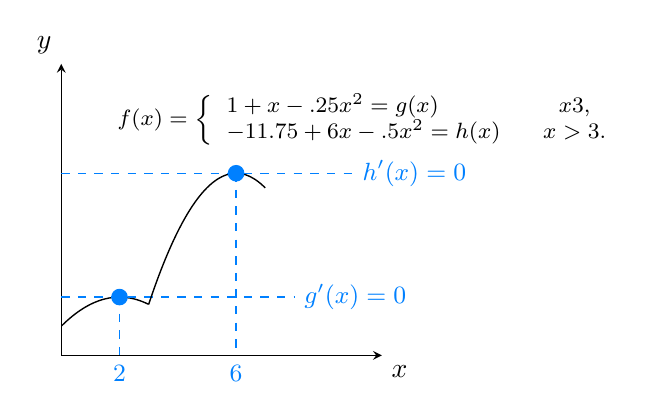
\begin{tikzpicture}[ 
axis/.style={very thick, ->, >=stealth'},
dashed line/.style={dashed, thin},
every node/.style={},
background rectangle/.style = {fill = gray90},
]
\begin{axis}[
  scale = .65,
  axis equal image, % forces a square plot
  clip = false, % allows plotting outside axis bounds
  axis x line=center, axis y line=center,
  xlabel = {$x$}, ylabel = {$y$},
  xtick={100}, ytick={100}, % effectively drops axis ticks
  xlabel style={below right}, ylabel style={above left},
  xmin=0, xmax=11,
  ymin=0, ymax=10]
\coordinate (origin) at (0, 0) ;
\path[name path=xaxis, gray] (0, 0) -- (10, 0);
\path[name path=yaxis, gray] (0, 0) -- (0, 10);
\coordinate (m1) at (4, 5) ;
% curves
\addplot [name path=X1curve, no marks, line width = .5pt, domain=0.01:3, smooth] {1+x-.25*x^(2)} node[above right, xshift = -1cm] (fend) {\small }; % f1x <- function(x) 4+x-.25*x^(2)
\coordinate (m1) at (2, 2);
\coordinate (m1Xaxis) at (m1 |- origin);
\coordinate (m1Yaxis) at (m1 -| origin);
\draw [name path=Horm1, azure, line width = .5pt, dashed] (m1Yaxis) -- ($(m1)+(6, 0)$) node[right] {\small $g'(x)=0$};
\draw [name path=Verm1, azure, line width = .5pt, dashed] (m1) -- (m1Xaxis) node[below] {\small $2$};
\fill [azure] (m1) circle (3pt);
\addplot [name path=X2curve, no marks, line width = .5pt, domain=3:7, smooth] {-11.75+6*x-.5*x^(2)} node[above right, xshift = -2cm, yshift = .4cm] (fend2) {\footnotesize $f(x)=
\left\{
\begin{array}{l}
1+x-.25x^{2}=g(x)\\
-11.75+6x-.5x^{2}=h(x)
\end{array}
\right. \ 
\begin{array}{c}
x\leqslant 3,\\
x>3.
\end{array}
$}; % f2x <- function(x) -11.75+6*x-.5*x^(2)
\coordinate (m2) at (6, 6.25);
\coordinate (m2Xaxis) at (m2 |- origin);
\coordinate (m2Yaxis) at (m2 -| origin);
\draw [name path=Horm2, azure, line width = .5pt, dashed] (m2Yaxis) -- ($(m2)+(4, 0)$) node[right] {\small $h'(x)=0$};
\draw [name path=Verm2, azure, line width = .5pt, dashed] (m2) -- (m2Xaxis) node[below] {\small $6$};
\fill [azure] (m2) circle (3pt);
\end{axis}
\end{tikzpicture}}\onslide<4->{\begin{tikzpicture}[ 
axis/.style={very thick, ->, >=stealth'},
dashed line/.style={dashed, thin},
every node/.style={},
background rectangle/.style = {fill = gray90},
]
\begin{axis}[
  scale = .7,
  axis equal image, % forces a square plot
  clip = false, % allows plotting outside axis bounds
  axis x line=center, axis y line=center,
  xlabel = {$x$}, ylabel = {$y$},
  xtick={100}, ytick={100}, % effectively drops axis ticks
  xlabel style={below right}, ylabel style={above left},
  xmin=0, xmax=11,
  ymin=0, ymax=10]
\coordinate (origin) at (axis cs: 0, 0) ;
\path[name path=xaxis, gray] (0, 0) -- (axis cs: 10, 0);
\path[name path=yaxis, gray] (0, 0) -- (axis cs: 0, 10);
\coordinate (m1) at (axis cs: 4, 5) ;
% curves
\addplot [name path=X3curve, no marks, line width = .5pt, domain=0.01:9, smooth] {8+.5*x-.4*x^(2)+(1/30)*x^(3)} node[above right, xshift = -1cm] (fend) {\small $f(x)=8+.5x-.4x^{2}+\tfrac{1}{30}x^{3}$};
%fx <- function(x) 8+.5*x-.4*x^(2)+(1/30)*x^(3)
\coordinate (m1) at (axis cs: 0.683370, 8.165525);
\coordinate (m2) at (axis cs: 7.316600, 3.301142);
\coordinate (m1Xaxis) at (m1 |- origin);
\coordinate (m2Xaxis) at (m2 |- origin);
\coordinate (m1Yaxis) at (m1 -| origin);
\coordinate (m2Yaxis) at (m2 -| origin);
\draw [name path=Horm1, azure, line width = .5pt, dashed] (m1Yaxis) -- ($(m1)+(axis cs: 4, 0)$) node[right] {\small $f'(x_{1})=0$};
\draw [name path=Verm1, azure, line width = .5pt, dashed] (m1) -- (m1Xaxis) node[below] {\small $.683$};
\draw [name path=Horm2, azure, line width = .5pt, dashed] ($(m2) + (axis cs: -2, 0)$) -- ($(m2)+(axis cs: 2, 0)$) node[right] {\small $f'(x_{2})=0$};
\draw [name path=Verm2, azure, line width = .5pt, dashed] (m2) -- (m2Xaxis) node[below] {\small $7.317$};
\fill [azure] (m1) circle (3pt) (m2) circle (3pt);
%\addplot[only marks, azure] coordinates {
%(0.683370, 8.165525)
%(7.316600, 3.301142)
%};
\end{axis}
\end{tikzpicture}
}

\vspace{-3ex}
\mpage{\paperwidth}{\onslide<3->{\mpage{.5\paperwidth}{\footnotesize 
$g'(x) = 1-.5x=0 \quad \Rightarrow \quad x = 2$\\
$h'(x) = 6-x=0 \quad \Rightarrow \quad x = 6$\\
 \hyperlink{DiffFormulae}{\beamergotobutton{微分公式}} $f(x)=bx^{n} \Rightarrow f'(x)=bnx^{n-1}$}}\onslide<4->{\mpage{.5\paperwidth}{$f'(x) = .5-.8x+.1x^{2}=0\\\quad \Rightarrow \quad x=4\pm 10\sqrt{.11}.$
 }}}

\vspace{-4cm}
\hspace{6.25cm}\onslide<4->{
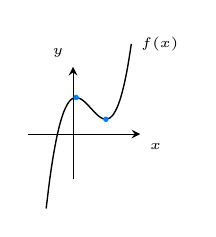
\begin{tikzpicture}[ 
axis/.style={very thick, ->, >=stealth'},
dashed line/.style={dashed, thin},
every node/.style={},
background rectangle/.style = {fill = gray90},
]
\begin{axis}[
  scale = .25,
  axis equal image, % forces a square plot
  clip = false, % allows plotting outside axis bounds
  axis x line=middle, axis y line=middle,
  xlabel = {\tiny $x$}, ylabel = {\tiny $y$},
  xtick={100}, ytick={100}, % effectively drops axis ticks
  xlabel style={below right}, ylabel style={above left},
  xmin=-10, xmax=15,
  ymin=-10, ymax=15]
\coordinate (origin) at (0, 0) ;
\path[draw = none, name path=xaxis, gray] (0, 0) -- (10, 0);
\path[draw = none, name path=yaxis, gray] (0, 0) -- (0, 10);
\coordinate (m1) at (4, 5) ;
% curves
\addplot [name path=X3curve, no marks, line width = .5pt, domain=-6:13, smooth] {8+.5*x-.4*x^(2)+(1/30)*x^(3)} node[right] (fend) {\tiny $f(x)$};%{\tiny $f(x)=8+.5x-.4x^{2}+\tfrac{1}{30}x^{3}$};
%fx <- function(x) 8+.5*x-.4*x^(2)+(1/30)*x^(3)
\coordinate (m1) at (axis cs: 0.683370, 8.165525);
\coordinate (m2) at (axis cs: 7.316600, 3.301142);
\fill [azure] (m1) circle (1pt) (m2) circle (1pt);
\end{axis}
\end{tikzpicture} 
}
\end{frame}

\begin{frame}[t]{}
\begin{dinglist}{45}
\vspace{1.0ex}\setlength{\itemsep}{1.0ex}\setlength{\baselineskip}{12pt}
\item	$f(x)=8+.5x-.4x^{2}+\tfrac{1}{30}x^{3}$のような3次関数は、最大値やと最小値が存在しません。最大値は無限大ですが、最大とか最小とかは有限の値のみに使います。よって、この関数には最大値も最小値も存在しないのです。しかし、極小値(局所的な最小値local minimum)や極大値(局所的な最大値local maximum)は存在します。右図の$x=7.317$は極小値、$x=.683$は極大値です。いずれも$f'(x)=0$が成り立ちます。
\pause
\item	以下では、関数が最大値(最小値)をもち、かつ、現在検討している$f'(x)=0$が関数の最大値(最小値)であると仮定し、そこでの数学的特徴を考えていきます。
\begin{dinglist}{43}
\vspace{1.0ex}\setlength{\itemsep}{1.0ex}\setlength{\baselineskip}{12pt}
\item	$f'(x)=0$が最大値(最小値)である確証を得るためには、一般的には関数をグラフにして全体を見渡す必要があります。
\end{dinglist}
\end{dinglist}
\end{frame}

\begin{frame}[t]{}
\begin{dinglist}{45}
\vspace{1.0ex}\setlength{\itemsep}{1.0ex}\setlength{\baselineskip}{12pt}
\item	一般に、$f'(x)=0$だけでは最大値か最小値か判定できません。最初の図で分かるように、最大値であれば最大値から外れると値が減っていきます。極値(最大値か最小値)なので関数の変化分$f'(x)$[=傾き]はゼロですが、傾きの変化は負値になります。
\pause
\item	傾きの変化は$f'(x)$をさらに微分した2階微分で計算できます。
	\begin{dinglist}{43}
	\vspace{1.0ex}\setlength{\itemsep}{1.0ex}\setlength{\baselineskip}{12pt}
\pause
	\item	2階微分は\textcolor{red}{加速度}を表します。
\pause
	\item	2階微分(加速度)が負とは、最初の図の$x>4$[``最大値の右側'']部分のように1階微分が負の関数では、傾きが率を高めて負値で小さくなっていく(絶対値では大きくなっていく)ことを意味します。よって、最大値の場合、2階微分は負$f''(x)<0$です。
\pause
	\item	1階微分が正の関数では、2階微分が負とは、正の傾きが率を高めて小さくなっていく(傾きは正のままゼロに近づいていく)ことを意味します。
	\end{dinglist}
\pause
\item	\textcolor{azure}{最大値ならば$f''(x)<0$}、\textcolor{azure}{最小値ならば$f''(x)>0$}というように、2階微分の符号で判定をします。ただし、2階微分がゼロ(=その地点で関数が線形=傾きが変化しない)の場合は、最大値か最小値か判定できません。
\end{dinglist}
\end{frame}

\begin{frame}[t]{}
\begin{dinglist}{43}
\vspace{1.0ex}\setlength{\itemsep}{1.0ex}\setlength{\baselineskip}{12pt}
\pause
\item	$f(x)=1+2x\textcolor{darkpastelgreen}{-}.25x^{2}\pause , f'(x)=2-.5x\pause , \textcolor{darkpastelgreen}{f''(x)=-.5<0}$. \pause よって、$f'(x)=2-.5x=0$が示す点は最\textcolor{darkpastelgreen}{大}化点。\pause $f(x)$を最大化する$x$は$f'(x)=2-.5x=0 \Rightarrow x=4.$
\pause
\item	$f(x)=1+2x\textcolor{darkpastelgreen}{+}.25x^{2}\pause , f'(x)=2+.5x\pause , \textcolor{darkpastelgreen}{f''(x)=.5>0}$.\pause  よって、$f'(x)=2+.5x=0$が示す点は最\textcolor{darkpastelgreen}{小}化点。\pause $f(x)$を最小化する$x$は$f'(x)=2+.5x=0 \Rightarrow x=-4.$
\end{dinglist}
\end{frame}

\begin{frame}[t]{}
\begin{columns}[T]
\column{.45\paperwidth}
例を考えます。2次関数(放物線)です。
\[
f(x)=1-2x^{2}+4x \Rightarrow f'(x)=-4x+4.
\]
\pause
$x$での接線の傾きは$-4x+4$です。仮に$x=2$だとしたら、接線の傾きは$f'(2)=-4*2+4=-4$です。最大化点を知るためには、接線の傾きがゼロの場所を探します。つまり、
\[
f'(x)=-4x+4=0
\]
を成立させる$x$を求めます。\pause
これはこの方程式を$x$について解けば得られます。
\[
x=1.
\]
\column{.45\paperwidth}
2階条件
\[
f''(x)=-4<0
\]
なので最大化点です。
最大化された値$f(1)=1-2+4=3$。% 近くの点で関数が3よりも小さいことを確認します。$f(0)=1$, $f(2)=1-8+8=1$。
\\~\\
\pause
次の例は1次関数(直線)です。
\[
f(x)=1+2x \Rightarrow f'(x)=2.
\]
\pause
$1+2x$は2の傾きで増えます。直線なので接線は関数そのものです。よって、接線の傾きは関数の傾きと同じ2です。直線なので最大化点は存在しません。よって、微分してゼロと置いても、$x=\cdots$と解くことはできません。
\end{columns}
\end{frame}

\begin{frame}[t]{}
参考: 微分できない場合1\\~\\
\onslide<2->{微分は関数の微小な変化を扱います。よって、(対象とする変数$x$の範囲で)関数が連続で滑らかでないと適用できません。\\~\\}
\onslide<3->{$x=a$で非連続である(ジャンプがある)と、$a$の前(左)の関数の値と$a$の後(右)の関数の値が異なります。行き着く先$x=a$で関数の値=極限の値=極値、が一致しないと、$x=a$で極値が存在しない、と言います。 $x=a$での微小な変化は、$a$での関数の極値を扱うので、極値が存在しないと議論できません。\\~\\}

\setbeamercovered{invisible}
\hfil\begin{tikzpicture}[ 
axis/.style={very thick, ->, >=stealth'},
dashed line/.style={dashed, thin},
every node/.style={},
wcircle/.style={circle, draw, color = azure, minimum size = 4pt, 
  inner sep = 0pt, outer sep = 0pt},
background rectangle/.style = {fill = gray90},
]
\begin{axis}[
  scale = .5,
  axis equal image, % forces a square plot
  clip = false, % allows plotting outside axis bounds
  axis x line=center, axis y line=center,
  xlabel = {$x$}, ylabel = {$y$},
  xtick={100}, ytick={100}, % effectively drops axis ticks
  xlabel style={below right}, ylabel style={above left},
  xmin=0, xmax=11,
  ymin=0, ymax=10]
\coordinate (origin) at (axis cs: 0, 0) ;
\path[name path=xaxis, gray] (0, 0) -- (axis cs: 10, 0);
\path[name path=yaxis, gray] (0, 0) -- (axis cs: 0, 10);
\coordinate (mx) at (axis cs: 5, 0) ;
\coordinate (m1) at (axis cs: 5, 6.75) ;
\coordinate (m2) at (axis cs: 5, 2.5) ;
% curves
\addplot [name path=f1curve,  no marks, line width = .5pt, domain=0.01:5, smooth] {1+.8*x-.1*x^(2)} node[below right] (f1end) {\small };
\addplot [name path=f2curve,  no marks, line width = .5pt, domain=5:9, smooth] {3+2*x-.25*x^(2)} node[right] (f2end) {\small f(x)};
\addplot [name path=Ver1, azure, no marks, line width = .5pt, domain=0.01:9, dashed, smooth] (5, 0) node [below]{$a$} -- (m1);
% jump point of curves
%\node [circle, draw, color = azure, fill=white] (b1) at (m1) {};
\fill [azure] (m2) circle (2pt);
\node [wcircle] at (m1) {} ;
\end{axis}
\end{tikzpicture}\begin{tikzpicture}[ 
axis/.style={very thick, ->, >=stealth'},
dashed line/.style={dashed, thin},
every node/.style={},
wcircle/.style={circle, draw, color = azure, minimum size = 4pt, 
  inner sep = 0pt, outer sep = 0pt},
background rectangle/.style = {fill = gray90},
]
\begin{axis}[
  scale = .5,
  axis equal image, % forces a square plot
  clip = false, % allows plotting outside axis bounds
  axis x line=center, axis y line=center,
  xlabel = {$x$}, ylabel = {$y$},
  xtick={100}, ytick={100}, % effectively drops axis ticks
  xlabel style={below right}, ylabel style={above left},
  xmin=0, xmax=11,
  ymin=0, ymax=10]
\coordinate (origin) at (axis cs: 0, 0) ;
\path[name path=xaxis, gray] (0, 0) -- (axis cs: 10, 0);
\path[name path=yaxis, gray] (0, 0) -- (axis cs: 0, 10);
% filled circles
\coordinate (m1) at (axis cs: 2, 2.5);
\coordinate (m2) at (axis cs: 4, 4) ;
\coordinate (m3) at (axis cs: 6, 6.5) ;
\coordinate (m4) at (axis cs: 8, 8) ;
% white circles
\coordinate (w1) at (axis cs: 2, 3.5);
\coordinate (w2) at (axis cs: 4, 6); 
\coordinate (w3) at (axis cs: 6, 7.5) ;
\coordinate (w4) at (axis cs: 8, 10) ;
% curves
\addplot [name path=s1curve, no marks, line width = .5pt, domain=0.01:2, smooth] {2+.25*x} node[below right] (s1end) {\small };
\addplot [name path=s2curve, no marks, line width = .5pt, domain=2:4, smooth] {3+.25*x} node[below right] (s2end) {\small };
\addplot [name path=s3curve, no marks, line width = .5pt, domain=4:6, smooth] {5+.25*x} node[below right] (s3end) {\small };
\addplot [name path=s4curve, no marks, line width = .5pt, domain=6:8, smooth] {6+.25*x} node[below right] (s4end) {\small };
\addplot [name path=s5curve, no marks, line width = .5pt, domain=8:10, smooth] {8+.25*x} node[below right] (s4end) {\small };
\addplot [name path=Ver1, azure, no marks, line width = .5pt, domain=1:9, dashed, smooth] (2, 0) node [below]{$2$} -- (m1);
\addplot [name path=Ver2, azure, no marks, line width = .5pt, domain=1:9, dashed, smooth] (4, 0) node [below]{$4$} -- (m2);
\addplot [name path=Ver3, azure, no marks, line width = .5pt, domain=1:9, dashed, smooth] (6, 0) node [below]{$6$} -- (m3);
\addplot [name path=Ver4, azure, no marks, line width = .5pt, domain=1:9, dashed, smooth] (8, 0) node [below]{$8$} -- (m4);
\addplot [name path=Hor2m, azure, no marks, line width = .5pt, domain=.01:9, dashed, smooth] (0, 4) node [left]{$4$} -- (m2);
\addplot [name path=Hor3w, azure, no marks, line width = .5pt, domain=.01:9, dashed, smooth] (0, 6) node [left]{$6$} -- (w2);
% jump point of curves
\node [wcircle] at (m1) {} 
node [wcircle] at (m2) {}
node [wcircle] at (m3) {}
node [wcircle] at (m4) {};
\fill [azure] (w1) circle (2pt) (w2) circle (2pt) (w3) circle (2pt) (w4) circle (2pt);
\node [xshift = 6cm] at (w2) {\mpage{6cm}{\footnotesize$
\left.
\begin{array}{l}
f(4)=6\\
\lim\limits_{x\uparrow 4}f(x)=4
\end{array}
\right\}
$ 非連続的ジャンプ}};
\end{axis}
\end{tikzpicture}
\end{frame}

\begin{frame}[t]{}
参考: 微分できない場合2\\~\\
\onslide<2->{$x=b$が尖っている(=滑らかでない)と、接線の傾きが左から$b$に近づく場合と右から$b$に近づく場合で異なるため、$x=b$での微小な変化の大きさが右と左で変わります。接線の傾きを1つに決められないために$x=b$で微分できません。下記の関数はそれ以外の点では微分可能です。\\~\\}

\setbeamercovered{invisible}
\hfil\begin{tikzpicture}[ 
axis/.style={very thick, ->, >=stealth'},
dashed line/.style={dashed, thin},
every node/.style={},
wcircle/.style={circle, draw, color = azure, minimum size = 4pt, 
  inner sep = 0pt, outer sep = 0pt},
background rectangle/.style = {fill = gray90},
]
\begin{axis}[
  scale = .5,
  axis equal image, % forces a square plot
  clip = false, % allows plotting outside axis bounds
  axis x line=center, axis y line=center,
  xlabel = {$x$}, ylabel = {$y$},
  xtick={100}, ytick={100}, % effectively drops axis ticks
  xlabel style={below right}, ylabel style={above left},
  xmin=0, xmax=11,
  ymin=0, ymax=10]
\coordinate (origin) at (axis cs: 0, 0) ;
\path[name path=xaxis, gray] (0, 0) -- (axis cs: 10, 0);
\path[name path=yaxis, gray] (0, 0) -- (axis cs: 0, 10);
\coordinate (mx) at (axis cs: 5, 0) ;
\coordinate (m1) at (axis cs: 5, 5) ;
% curves
\addplot [name path=f1curve,  no marks, line width = .5pt, domain=0.01:5, smooth] {3+.4*x} node[below right] (f1end) {\small };
\addplot [name path=f2curve,  no marks, line width = .5pt, domain=5:9, smooth] {-2.5+1.5*x} node[right] (f2end) {\small f(x)};
\addplot [name path=Ver, azure, no marks, line width = .5pt, dashed, smooth] (5, 0) node [below]{$b$} -- (m1);
\draw [azure, <-, latex-] ($(m1) + (.5, 0)$) -- ++(3, 0) node[azure, right]{\footnotesize kink}; 
\end{axis}
\end{tikzpicture}

\begin{itemize}\footnotesize
\vspace{1.0ex}\setlength{\itemsep}{1.0ex}\setlength{\baselineskip}{12pt}
\onslide<3->{
\item	$b$での左部分での微分を左右からの微分left differentiationと呼びます。$b$での右部分での微分を右からの微分right differentiationと呼びます。
}
\onslide<4->{
\item	微分できない点なのに、右からの微分とか左からの微分とかいう用語法は、厳密には矛盾しています。詳しい事情は知りません。
}
\end{itemize}
\end{frame}

\begin{frame}[t, label=DiffFormulae]{}
1変数関数$f(x)$の微分の公式\\
\renewcommand{\arraystretch}{1.2}
\setlength{\tabcolsep}{1pt}
\begin{tabular}{
>{\hfill$}p{4cm}<{$}
>{\hfil$}p{.75cm}<{$}
>{$}p{5.5cm}<{$\hfill}
>{\footnotesize}p{5cm}<{\hfill}
}
f(x)=a &\textcolor{red}{\Rightarrow} &\textcolor{azure}{f'(x)=0} & 水平線の傾きは0\\
f(x)=bx^{n} &\textcolor{red}{\Rightarrow} & \textcolor{azure}{f'(x)=bnx^{n-1}}& 指数関数、$n=1$は線形関数\\
f(x)=\frac{b}{x^{n}}=bx^{-n} &\textcolor{red}{\Rightarrow} & f'(x)=-bnx^{-n-1}& 分数は指数関数の一種\\
f(x)=g(x)+h(x)&\textcolor{red}{\Rightarrow} & \textcolor{azure}{f'(x)=g'(x)+h'(x)}& 和の微分公式\\
f(x)=g(x)h(x)&\textcolor{red}{\Rightarrow} & \textcolor{azure}{f'(x)=g'(x)h(x)+g(x)h'(x)}& 積の微分公式\\
f(x)=g\left\{h(x)\right\}&\textcolor{red}{\Rightarrow} & \textcolor{azure}{f'(x)=g'(h)h'(x)}& チェーンルール\\
f(x)=b\ln x &\textcolor{red}{\Rightarrow} & f'(x)=b\frac{1}{x}& 対数関数の微分公式\\
f(x)=ae^{bx} &\textcolor{red}{\Rightarrow} & f'(x)=abe^{bx} & 自然指数関数の微分公式
\end{tabular}

\hfill\hyperlink{fx<5>}{\beamergotobutton{戻る}}
\end{frame}

\begin{frame}[t]{}
参考: なぜ$f'(x)=bnx^{n-1}$?\\~\\
証明ではないですが、定義を使って計算すると公式の正しさが確認できます。微分の定義は以下です。関数の変化(率の極限)を求めています。
\[
f'(x)=\lim_{h\rightarrow 0}\frac{f(x+h)-f(x)}{h}.
\]
\pause
$f(x)=a+bx+cx^{2}$で考えます。$f'(x)=bnx^{n-1}=b+2cx$。定義を使うと
\[
\begin{aligned}
\lim_{h\rightarrow 0}\frac{f(x+h)-f(x)}{h}
&=
\lim_{h\rightarrow 0}\frac{a+b(x+h)+c(x+h)^{2}-(a+bx+cx^{2})}{h},\\
&=
\lim_{h\rightarrow 0}\frac{a+b(x+h)+c(x^{2}+2hx+h^{2})-(a+bx+cx^{2})}{h},\\
&=
\lim_{h\rightarrow 0}\frac{bh+2chx+h^{2}}{h},\\
&=
\lim_{h\rightarrow 0}b+2cx+h,\\
&=
b+2cx.
\end{aligned}
\]
\end{frame}

\begin{frame}[t]{}
参考: なぜ$f'(x)=bnx^{n-1}$?\\~\\
証明のスケッチ: $f(x)=a+bx+cx^{2}+\cdots+dx^{n}$で考えます。$f'(x)=b+2cx+\cdots+dnx^{n-1}$。定義を使うと
\[
\begin{aligned}
\lim_{h\rightarrow 0}&\frac{f(x+h)-f(x)}{h}\\
&=
\lim_{h\rightarrow 0}\frac{a+b(x+h)+c(x+h)^{2}+\cdots+d(x+h)^{n}-(a+bx+cx^{2}+\cdots+dx^{n})}{h},\\
&=
\lim_{h\rightarrow 0}\bigg(\frac{a+b(x+h)+c(x^{2}+2hx+h^{2})+\cdots+d(x^{n}+nhx^{n-1}+\cdots+h^{n})}{h},\\
&\hspace{4em}-\frac{a+bx+cx^{2}+\cdots+dx^{n}}{h}\bigg),\\
&=
\lim_{h\rightarrow 0}\frac{bh+2chx+ch^{2}+\cdots+d(nhx^{n-1}+nh^{2}x^{n-2}+\cdots+h^{n})}{h},\\
&=
b+2cx+\cdots+dnx^{n-1}.
\end{aligned}
\]
\end{frame}

\begin{frame}[t, label=ChainRule]{}
チェーンルール
\begin{columns}[T]
\column{.4\textwidth}
\onslide<1->{\[
\begin{aligned}
f(x)
&=
g\left\{h(x)\right\}\\ 
&\textcolor{red}{\Rightarrow}\quad \textcolor{azure}{f'(x)=g'(h)h'(x)}.
\end{aligned}
\]
$f(x)$が$g\{h(x)\}$という$g(h)$, $h(x)$の二重の関数になっている場合:
}
\begin{enumerate}
\vspace{1.0ex}\setlength{\itemsep}{1.0ex}\setlength{\baselineskip}{12pt}
\onslide<3->{\item	$h$を変数のように考えて$g(h)$を$h$で微分: $g'(h)$}
\onslide<4->{\item	$h(x)$を$x$で微分: $h'(x)$}
\onslide<5->{\item	両方を乗じた$g'(h)h'(x)$が全体$f(x)$の微分となる\\[2ex]}
\end{enumerate}
\[
\onslide<6->{x\mbox{が変化}}
\onslide<7->{\underbrace{\rightarrow h\mbox{が変化}}_{\textcolor{aqua}{h'(x)}}}
\onslide<8->{\underbrace{\rightarrow g\mbox{が変化}}_{\textcolor{aqua}{g'(h)}}}
\]
\column{.6\textwidth}
\onslide<9->{
$g(h)=2h+1, h(x)=2x^{2}+x-1$の場合\\
$f(x)=g\{h(x)\}=2(2x^{2}+1x-1)+1$\\
}
\onslide<10->{$g'(h)=2$, $h'(x)=4x+1$}
\onslide<11->{なので、$f'(x)=g'(h)h'(x)=2\times (4x+1)=8x+2$. }
\onslide<12->{$f(x)=g\{h(x)\}=2(2x^{2}+1x-1)+1=4x^{2}+2x-1$だから、微分すると$f'(x)=8x+2$で同じになることが確認できる。\\~\\}
\end{columns}
\end{frame}

\begin{frame}[t]{}
\begin{columns}[T]
\column{.5\textwidth}
$f(l)=\beta u\{h(l)+Rs\}$で$f(l)=\beta u\{c_{2}(l)\}=g\left\{c_{2}(l)\right\}$、つまり、$g(c_{2})=\beta u(c_{2})$, $c_{2}(l)=h(l)+Rs$とおく
\[
g'(c_{2})=\beta u'(c_{2}), \; c_{2}'(l)=h'(l).
\]
チェーンルール
\[
\begin{aligned}
f(l)
&=
g\left\{c_{2}(l)\right\},\\
f'(l)
&=
g'(c_{2})c'_{2}(l),\\
&=
\beta u'(c_{2})h'(l),\\
&=
\beta u'\{h(l)+Rs\}h'(l).
\end{aligned}
\]
\pause
$g, h$を微分して乗じても手数は変わらないですが、計算の誤りが減ります。
\column{.5\textwidth}
\pause
2変数の関数$u\left\{w(24-l)+A-s\right\}+\beta u\{h(l)+Rs\}$を2変数$l, s$で最大化

\pause
{\tiny \textcolor{green}{1.} $l$について\textcolor{green}{偏微分}してゼロとおく \; \textcolor{green}{2.} $s$について\textcolor{green}{偏微分}してゼロとおく}

\pause
$F(l, s)=u\left\{c_{1}(l, s)\right\}+\beta u\{c_{2}(l, s)\}$、つまり、$c_{1}(l, s)=w(24-l)+A-s$, $c_{2}(l, s)=h(l)+Rs$
\pause
{\small
\[
\begin{aligned}
F_{l}(l, s)
&=
u'\left(c_{1}\right)c_{1l}(l, s)+\beta u'(c_{2})c_{2l}(l, s)=0,\\
F_{s}(l, s)
&=
u'\left(c_{1}\right)c_{1s}(l, s)+\beta u'(c_{2})c_{2s}(l, s)=0.
\end{aligned}
\]
}
\[
\begin{aligned}
\frac{u'\left(c_{1}\right)}{u'\left(c_{2}\right)}&=-\beta \frac{c_{2l}(l, s)}{c_{1l}(l, s)}, \\
\frac{u'\left(c_{1}\right)}{u'\left(c_{2}\right)}&=-\beta \frac{c_{2s}(l, s)}{c_{1s}(l, s)}. 
\end{aligned}
\]
\end{columns}
\end{frame}

\begin{frame}[t]{}
$F(l, s)=u\left\{w(24-l)+A-s\right\}+\beta u\{h(l)+Rs\}$を2変数$l, s$で最大化

\pause
{\scriptsize 1. $l$について偏微分してゼロとおく \; 2. $s$について偏微分してゼロとおく}
\[
\begin{aligned}
\frac{\partial F(l, s)}{\partial l}
&=
\frac{\partial u\left(c_{1}\right)}{\partial c_{1}}\frac{\partial c_{1}(l, s)}{\partial l}
+\beta \frac{\partial u(c_{2})}{\partial c_{2}}\frac{\partial c_{2}(l, s)}{\partial l}=0, 
\pause
\quad 
&\frac{\frac{\partial u\left(c_{1}\right)}{\partial c_{1}}}{\frac{\partial u\left(c_{2}\right)}{\partial c_{2}}}
&=
-\beta \frac{\frac{\partial c_{2}(l, s)}{\partial l}}{\frac{\partial c_{1}(l, s)}{\partial l}},\\
\pause
\frac{\partial F(l, s)}{\partial s}
&=
\frac{\partial u\left(c_{1}\right)}{\partial c_{1}}\frac{\partial c_{1}(l, s)}{\partial s}
+\beta \frac{\partial u(c_{2})}{\partial c_{2}}\frac{\partial c_{2}(l, s)}{\partial s}=0, 
\pause
\quad
&\frac{\frac{\partial u\left(c_{1}\right)}{\partial c_{1}}}{\frac{\partial u\left(c_{2}\right)}{\partial c_{2}}}
&=
-\beta \frac{\frac{\partial c_{2}(l, s)}{\partial s}}{\frac{\partial c_{1}(l, s)}{\partial s}}.
\end{aligned}
\]

\begin{columns}[T]
\column{.7\textwidth}
\pause
$c_{1}(l, s)=w(24-l)+A-s$\pause, $\frac{\partial c_{1}(l, s)}{\partial l}=-w$, $\frac{\partial c_{1}(l, s)}{\partial s}=-1$, 

\pause
$c_{2}(l, s)=h(l)+Rs$\pause, $\frac{\partial c_{2}(l, s)}{\partial l}=h'(l)$, $\frac{\partial c_{2}(l, s)}{\partial s}=R$.

\vspace{-1ex}
\pause
\[
\begin{aligned}
\frac{u'\left(c_{1}\right)}{u'\left(c_{2}\right)}&=
\frac{\frac{\partial u\left(c_{1}\right)}{\partial c_{1}}}{\frac{\partial u\left(c_{2}\right)}{\partial c_{2}}}
\pause
=
-\beta \frac{\frac{\partial c_{2}(l, s)}{\partial l}}{\frac{\partial c_{1}(l, s)}{\partial l}}
\pause
=-\beta\frac{h'(l)}{-w}=\beta\frac{h'(l)}{w},\\
\pause
\frac{u'\left(c_{1}\right)}{u'\left(c_{2}\right)}&=
\frac{\frac{\partial u\left(c_{1}\right)}{\partial c_{1}}}{\frac{\partial u\left(c_{2}\right)}{\partial c_{2}}}
\pause
=
-\beta \frac{\frac{\partial c_{2}(l, s)}{\partial s}}{\frac{\partial c_{1}(l, s)}{\partial s}}
\pause
=-\beta\frac{R}{-1}=\beta R. 
\end{aligned}
\]
\column{.3\textwidth}
\pause
\[
wR=h'(l).
\]
$F(l, s)$を2変数$l, s$で最大化すると、この条件が成り立っていなければならない

\pause
限界収益が時間の2使途で同じ
\end{columns}
\end{frame}

\begin{frame}{}
純便益=粗便益-費用です。
\pause
粗便益も費用も$x$の関数だとしましょう。粗便益$b(x)$、費用$c(x)$と関数表記します。
\pause 
経済学では2階微分の符号を以下のように仮定することが多いです。
\[
b'(x) > 0, \quad b''(x)<0, \quad c'(x)>0, \quad c''(x)>0 \; \mbox{for all }x\in\mathbb R_{+}.
\]
\begin{dinglist}{43}
\vspace{1.0ex}\setlength{\itemsep}{1.0ex}\setlength{\baselineskip}{12pt}
\pause 
\item	$\in$は``is in'', ``belongs to''と読みます。
\pause 
\item	$\mathbb R_{+}$は0を含む正の実数(real numbers)全ての集合のことです。\\[2ex]
\end{dinglist}
\pause 
よって、「$\mbox{for all }x\in\mathbb R_{+}$」とは「for all $x$ in the set of all positive real numbers」($x$は正の実数すべての集合、もしくは、$x$は正の実数であれば何でもよい)と読みます。\pause つまり、$x$が正の実数であれば、1階微分と2階微分の符号がこのようになる、と書いています。
\begin{dinglist}{43}
\vspace{1.0ex}\setlength{\itemsep}{1.0ex}\setlength{\baselineskip}{12pt}
\pause 
\item	例として$x$は時間や生産量と考え、正の実数しか取り得ない状況を考えます。
\end{dinglist}

\vspace{2ex}
\pause 
経済学では$b'(x)$を\textcolor{red}{限界便益marginal benefits}、$c'(x)$を\textcolor{red}{限界費用marginal costs}と呼びます。
\end{frame}

\begin{frame}{}
純便益$=b(x)-c(x)$を最大化するには、微分してその値をゼロとおきます。つまり、最大値では
\[
b'(x)-c'(x)=0
\]
が成り立っています。これが成り立たないところは最大値ではありません。
	\begin{dinglist}{43}
	\vspace{1.0ex}\setlength{\itemsep}{1.0ex}\setlength{\baselineskip}{12pt}
\pause
	\item	\textcolor{red}{限界便益=限界費用}
\end{dinglist}
\pause
\vspace{2ex}
一階微分がゼロ(一階条件first order condition)だけだと最小値かもしれません。2階微分が負(最大値の二階条件second order condition for the maximum)か確認します。
\[
b''(x)-c''(x)<0. \quad \Leftarrow \quad b''(x)<0, \ c''(x)>0 \ \mbox{for all }x\in\mathbb R_{+}.
\]
\begin{dinglist}{45}
\vspace{1.0ex}\setlength{\itemsep}{1.0ex}\setlength{\baselineskip}{12pt}
\pause
	\item	$x$は正の実数なので0という下限値があります。ここでは関数の最大値が下限値$x=0$ではない、と(説明なく)仮定しています。実は、最大値が$x=0$の場合、一階条件は$b'(x)-c'(x)\leqslant 0$となるのですが、この点は後で説明します。
\pause
	\item	最大化問題が解を持つように、以下も成り立つと仮定します。この意味は後で図を使って説明します。
	\[
	\mbox{\footnotesize \textcolor{azure}{[$b'(x)$の$Y$切片]}} \lim_{x\rightarrow 0}b'(x)=g, \quad \mbox{\footnotesize \textcolor{azure}{[$c'(x)$の$Y$切片]}} \lim_{x\rightarrow 0}c'(x)=h, \quad g>h.
	\]
	\end{dinglist}
\end{frame}

\begin{frame}{}
\begin{columns}[T]
\column{.4\textwidth}
\hfil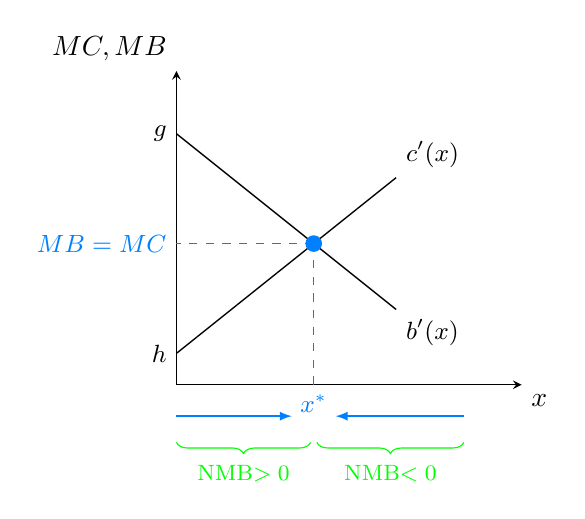
\begin{tikzpicture}[ 
axis/.style={very thick, ->, >=stealth'},
dashed line/.style={dashed, thin},
every node/.style={},
background rectangle/.style = {fill = gray90},
]
\begin{axis}[
  scale = .7,
  axis equal image, % forces a square plot
  clip = false, % allows plotting outside axis bounds
  axis x line=center, axis y line=center,
  xlabel = {$x$}, ylabel = {$MC, MB$},
  xtick={100}, ytick={100}, % effectively drops axis ticks
  xlabel style={below right}, ylabel style={above left},
  xmin=0, xmax=11,
  ymin=0, ymax=10]
\coordinate (origin) at (axis cs: 0, 0) ;
\path[name path=xaxis, gray] (0, 0) -- (axis cs: 10, 0);
\path[name path=yaxis, gray] (0, 0) -- (axis cs: 0, 10);
% curves
\addplot [name path=MBcurve, no marks, line width = .5pt, domain=0.01:7, smooth] {8-.8*x} node[below right] (MBend) {\small $b'(x)$};
\addplot [name path=MCcurve, no marks, line width = .5pt, domain=0.01:7, smooth] {1+.8*x} node[above right] (MCend) {\small $c'(x)$};
% intersection, x and y coordinates of intersections
\path [name intersections={of=MBcurve and MCcurve, by={e1}}];
\coordinate (e1Xaxis) at (e1 |- origin) ;
\coordinate (e1Yaxis) at (e1 -| origin);
\coordinate (MBendXaxis) at (MBend |- origin);
\draw [name path=Hor1, azure, line width = .5pt, dashed] (e1) -- (e1Yaxis) node[left] {\small $MB=MC$};
\draw [name path=Ver1, azure, line width = .5pt, dashed] (e1)  -- (e1Xaxis) node[below] {\small $x^{*}$};
% curly braces
\draw [decorate, green, decoration={brace, mirror, raise = 1pt, amplitude=4pt}, xshift=0cm, yshift=0pt]
  ($(origin)+ (0, -1.75)$) -- ($(e1Xaxis) + (-.1, -1.75)$) 
  node (MNBplus) [midway, green, below, yshift = -.2cm, xshift=.0cm] {\footnotesize NMB$>0$}; 
\draw [decorate, green, decoration={brace, mirror, raise = 1pt, amplitude=4pt}, xshift=0cm, yshift=0pt]
  ($(e1Xaxis) + (.1, -1.75)$) -- ($(MBendXaxis) + (1, -1.75)$) 
  node (MNBnegative) [midway, green, below, yshift = -.2cm, xshift=.0cm] {\footnotesize NMB$<0$}; 
% arrows to x*
\draw [name path=rangeMNBplus, azure, line width = .5pt, ->, -latex, yshift = -.5cm] ($(origin)+ (0, -1)$) -- ($(e1Xaxis) + (-.7, -1)$);
\draw [name path=rangeMNBnegative, azure, line width = .5pt, <-, latex-, yshift = -.5cm]  ($(e1Xaxis) + (.7, -1)$) -- ($(MBendXaxis) + (1, -1)$);
% intersections of curves
\fill [azure] (e1) circle (3pt);
\draw (axis cs: 0, 8) node[left] {\small $g$};
\draw (axis cs: 0, 1) node[left] {\small $h$};
\end{axis}
\end{tikzpicture}
\column{.6\textwidth}
\begin{dinglist}{45}
\vspace{1.0ex}\setlength{\itemsep}{1.0ex}\setlength{\baselineskip}{12pt}
\pause
\item	Second order conditions: $b''(x)<0, c''(x)>0$
\pause
\item	$b''(x)$は$b'(x)$の$x$に対する傾きです。$b''(x)<0$なので$b'(x)$は右下がりです。
\pause
\item	この図で限界便益と限界費用の差$b'(x)-c'(x)$、つまり、縦方向の長さが限界純便益net marginal benefits (NMB)です。限界純便益とは、$x$を変化することによる純便益変化の大きさです。
\pause
\item	最大値の二階条件(限界便益-限界費用は$x$が増えると減る)が満たされているので、限界純便益が正であれば、$x$を増やすと純便益が増えます。限界純便益が負であれば、$x$を減らすと純便益が増えます。
\end{dinglist}
\end{columns}
\pause
{\footnotesize
\[
\left.\begin{aligned}
b''(x)&<0 \mbox{ for all }x\in\mathbb R_{+} &&[\Leftrightarrow &&b'(x)\mbox{は減少関数],} && \lim_{x\rightarrow 0}b'(x)=g,\\
c''(x)&>0 \mbox{ for all }x\in\mathbb R_{+} &&[\Leftrightarrow &&c'(x)\mbox{は増加関数],} && \lim_{x\rightarrow 0}c'(x)=h,
\end{aligned}
\quad g>h
\ \right\}
\ \mbox{\mpagethree{3.5cm}{なので$x$が正の領域で\\ 交点がある}{c}}
\]
}
\end{frame}

\begin{frame}[t]{}
%\hfil\adjustbox{max height=.3\paperheight}{
\input{c:/seiro/docs/external/seishin/lec_slides/2024/MaximisationSlides/NonnegativityConstraint.tex}\\
%}
\vspace{1.0ex}
$x=0$が最大値となる場合は上図の右2つのケースです。
\begin{itemize}
\vspace{1.0ex}\setlength{\itemsep}{1.0ex}\setlength{\baselineskip}{12pt}
\pause
\item	中央の図は最大値を与える$x$が負です。$x$は時間ですから、負の時間など無いので、最大化点は$x$が取り得る最も小さい値の0となります。
	\begin{dinglist}{43}
	\vspace{1.0ex}\setlength{\itemsep}{1.0ex}\setlength{\baselineskip}{12pt}
	\pause
	\item	$x$が負値を取れない状況: 「非負制約nonnegativity constraintがある」\\[2ex]
	\end{dinglist}
\textcolor{red}{非負制約がbindしていると最大値での接線$f'(x)$の傾きが負}になります。
\pause
\item	右の図は$x=0$のときに関数が最大化されている場合です。この状況では非負制約を考えずに最大化問題を$f'(x)=0$で解いても$x^{*}=0$となります。%このときの最大化点での接線の傾きはゼロです。
\pause
\item	左の図は非負制約が縛りを課さない(bindしない、nonbinding)ケースです。\\[2ex]
\end{itemize}
\end{frame}

\begin{frame}[t]{}
\input{c:/seiro/docs/external/seishin/lec_slides/2024/MaximisationSlides/NonnegativityConstraint.tex}
\begin{dinglist}{43}
\vspace{1.0ex}\setlength{\itemsep}{1.0ex}\setlength{\baselineskip}{12pt}
\pause
\item	非負制約つきの最大化問題の解は、関数の形状によって上図3つのいずれかになります。
\pause
\item	非負制約がbindしていれば接線の傾きは負、bindしていなければゼロなので、非負制約つき最大化問題の解では、目的関数(純便益関数)の傾きが負かゼロ、つまり、非正であること、$f'(x)\leqslant 0$が必要です(これが非負制約つき最大化問題の一階条件first order conditionです)。
\pause
%\item	中央や右の図の場合、遠隔授業をせず、すべてを対面授業にすれば社会の純便益を最大化できます。
\end{dinglist}
\end{frame}

\begin{frame}[t]{}
交差微分cross derivatives: 資本と労働を要素とする生産関数を考えます。
\[
Y=AF(K, L). \quad \textcolor{azure}{\footnotesize Y=K^{.3}L^{.7}}
\]
\pause
$L$について微分すると
\[
\frac{\partial Y}{\partial L}=A\frac{\partial F(K, L)}{\partial L}=AF_{L}(K, L). \pause
\quad \textcolor{azure}{\footnotesize F_{L}=.7\left(\frac{K}{L}\right)^{.3}}
\]
\pause
$F_{L}(K, L)$は$\frac{\partial F(K, L)}{\partial L}$の簡易表示です。一般に、$F_{L}(K, L)$は$K$と$L$の関数です。$F(K, L)$が連続して微分可能と仮定すると、$F_{L}(K, L)$を$L$で微分すると$F_{LL}(K, L)$、$K$で微分すると$F_{LK}(K, L)$が得られます。\\~\\
%$F_{LL}(K, L)$は$L$に関する2階微分です。\\~\\
\pause
$F_{LK}(K, L)$は$L$に関する微分$F_{L}(K, L)$を$K$で(交差して)微分するので、交差微分といいます。\pause
$F_{LK}=F_{KL}$であることが証明できます。\\~\\
\pause
$F_{LK}(K, L)$は$F_{L}(K, L)$が$K$とともに変化する方向(正=増える、負=減る)です。\\~\\
\pause
多くの生産関数は$F_{LK}(K, L)>0$です。資本$K$が増えると労働の限界生産性$F_{L}(K, L)$は増えることが多いためです。\pause
\textcolor{azure}{\footnotesize $F_{LK}=.7*.3\frac{1}{K^{.7}L^{.3}}>0.$ $F_{L}$は$K$の増加関数。}
\end{frame}

\begin{frame}[t]{}
おまけ: 全微分=関数のすべての変数について微分すること\\~\\
資本と労働を要素とする生産関数を考えましょう。
\[
Y=AF(K, L).
\]
全微分すると(積の公式)
\[
dY=F(K, L)dA+A\frac{\partial F}{\partial K}dK+A\frac{\partial F}{\partial L}dL.
\]
両辺をそれぞれ$Y$と$AF(K, L)$で割ると
\[
\frac{dY}{Y}=\frac{dA}{A}+\frac{F_{K}dK}{F(K, L)}+\frac{F_{L}dL}{F(K, L)}.
\]
\end{frame}

\begin{frame}[t]{}
おまけ: $Y=AF(K, L)=AK^{\alpha}L^{1-\alpha}, \quad \alpha\in(0, 1)$をコブ・ダグラス型生産関数といいます。最もよく使われる生産関数形の1つです。
\[
\begin{aligned}
Y
&=
AF(K, L)=AK^{\alpha}L^{1-\alpha}, \quad \alpha\in(0, 1), \ F_{K}=\alpha K^{\alpha-1}L^{1-\alpha}, F_{L}=(1-\alpha)K^{\alpha}L^{-\alpha},\\
\frac{dY}{Y}
&=
\frac{dA}{A}+\alpha K^{-1}dK+(1-\alpha)L^{-1}dL=
\frac{dA}{A}+\alpha\frac{dK}{K}+(1-\alpha)\frac{dL}{L}.\\
\hat{Y}
&=
\hat{A}+\alpha\hat{K}+(1-\alpha)\hat{L}.
\end{aligned}
\]
労働生産性$y=\frac{Y}{L}$の変化率を計算します。
\[
\begin{aligned}
y
&=
\frac{Y}{L}
=
AK^{\alpha}L^{-\alpha}=A\left(\frac{K}{L}\right)^{\alpha}=Ak^{\alpha}, \quad k=\frac{K}{L}\quad\Rightarrow\quad
\frac{dy}{y}
=
\frac{dA}{A}+\alpha\frac{dk}{k}.\\
\hat{y}
&=
\hat{A}+\alpha\hat{k}.
\end{aligned}
\]
よって、労働生産性の成長率はTFP成長率と$\alpha\times$労働1単位あたり資本成長率(=資本深化)に分解できます。
\end{frame}

\begin{frame}[t]{}
おまけ: コブ・ダグラス型生産関数の$\alpha$は資本分配率パラメタといい、資本分配率($=rK/pY$)に等しくなる、と示すことができます。\\~\\
利潤最大化問題
\[
\max_{\{K, L\}}\pi=pAK^{\alpha}L^{1-\alpha}-rK-wL, \quad \alpha\in(0, 1).
\]
$K$についてのFOCは
\[
pA\alpha K^{\alpha-1}L^{\alpha}-r=0 \quad \Rightarrow \quad r=MPK=\alpha \frac{pAK^{\alpha}L^{1-\alpha}}{K}=\alpha \frac{pY}{K}.
\]
よって、$\alpha$は資本報酬/収入の比に等しい。
\[
\alpha=\frac{rK}{pY}.
\]
別の言い方をすれば、コブ・ダグラス型生産関数では、資本報酬$=\alpha\times$収入が成り立つ。
\end{frame}

\begin{frame}[t]{}
おまけ: $L$についてのFOCは
\[
pA(1-\alpha) K^{\alpha}L^{\alpha-1}-w=0 \quad \Rightarrow \quad w=MPL=(1-\alpha) \frac{pAK^{\alpha}L^{1-\alpha}}{L}=(1-\alpha) \frac{pY}{L}.
\]
$1-\alpha$は労働分配率に等しくなります。
\[
1-\alpha=\frac{wL}{pY}.
\]
FOCsを$K, L$について解くと
\[
K^{*}=\alpha \frac{pY}{r}, \quad L^{*}=(1-\alpha)\frac{pY}{w}.
\]
解$K^{*}, L^{*}$を目的関数(利潤)に代入すると、最大化された利潤は0であることが分かります。
\[
\pi^{*}=pY-r\alpha \frac{pY}{r}-w(1-\alpha)\frac{pY}{w}=pY-pY=0.
\]
コブ・ダグラス型生産関数では、価格$p, w, r$を所与とした完全競争下の利潤最大化では、収入$pY$は資本と労働に完全分配されて利潤が0になります。
% FOCsを比に取ると
% \[
% \frac{w}{r}=\frac{MPL}{MPK}=
% \frac{(1-\alpha) \frac{pY}{L}}{\alpha \frac{pY}{K}}=\frac{1-\alpha}{\alpha}\frac{K}{L},
% \]
% もしくは
% \[
% \alpha wL=
% (1-\alpha)rK.
% \]
\end{frame}

\begin{frame}[t]{}
おまけ: $A$が誤差付きの$\tilde{A}$として測定されるとき
\[
\tilde{A}=a+bA.
\]
$a, b$は変化しない定数だとします。TFP成長率は$\frac{dA}{A}$として計算されます。ここで計測されるのは$\tilde{A}$なので、$\frac{d\tilde{A}}{\tilde{A}}$を計算することになります。微分すると定数は0になるので
\[
d\tilde{A}=bdA.
\]
よって
\[
\frac{d\tilde{A}}{\tilde{A}}=\frac{bdA}{a+bA}=\frac{dA}{\frac{a}{b}+A}.
\]
つまり、$a=0$であれば$\frac{d\tilde{A}}{\tilde{A}}=\frac{dA}{A}$です。
\end{frame}

\begin{frame}[t]{}
まとめ
\begin{itemize}
\vspace{1.0ex}\setlength{\itemsep}{3.0ex}\setlength{\baselineskip}{12pt}
\item	関数を最大化(最小化)するには微分してゼロとおき$f'(x)=0$、その方程式で$x$について解く。
	\begin{dinglist}{43}\footnotesize
	\vspace{1.0ex}\setlength{\itemsep}{1.0ex}\setlength{\baselineskip}{12pt}
\pause
	\item	微分できない関数もある。
\pause
	\item	2階条件[$f''(x)$の符号]で最大値か最小値か判明する。
\pause
	\item	微分できて2階条件が最大化(最小化)であっても、他に最大化点(最小化点)がある可能性がある。一般にはグラフ化して確認する必要がある。
	\end{dinglist}
\pause
\item	純便益関数の最大化で、純便益関数が便益関数-費用関数と2つに分離できる場合は、最大化点は限界便益=限界費用が成立する点。
	\begin{dinglist}{43}\footnotesize
	\vspace{1.0ex}\setlength{\itemsep}{1.0ex}\setlength{\baselineskip}{12pt}
\pause
	\item	限界便益=限界費用は限界便益線と限界費用線が交差する点。
\pause
	\item	交差するためには、限界便益が右下がり、限界費用が右上がり、$x$が小さいときに限界便益$>$限界費用、という条件が必要。
	\end{dinglist}
\pause
\item	$x$に非負制約があるとき、$x=0$が最大化点の場合もある。その場合は$f'(0)\leqslant 0$が成立している。
\end{itemize}
\end{frame}

\end{document}

\begin{frame}[t]{}
\begin{columns}[T]
\column{.5\textwidth}
$f(l)=u\left\{w(24-l)+A-s\right\}+\beta u\{h(l)+Rs\}$で
\pause
$f(l)=u\left\{c_{1}(l)\right\}+\beta u\{c_{2}(l)\}$、つまり、$c_{1}(l)=w(24-l)+A-s$, $c_{2}(l)=h(l)+Rs$とおく
\pause
チェーンルール
\[
\begin{aligned}
f'(l)
&=
u'\left(c_{1}\right)c'_{1}(l)+g'(c_{2})c'_{2}(l),\\
&=
u'\left(c_{1}\right)*(-w)+\beta u'(c_{2})h'(l),\\
&=
0
\end{aligned}
\]
$\Leftrightarrow$
\[
\frac{u'\left(c_{1}\right)}{u'\left(c_{2}\right)}=\beta \frac{h'(l)}{w}.
\]
\column{.5\textwidth}
$w(24-l)+A-s=c_{1}$のとき、普通の微分をして0とおく
\[
\begin{aligned}
U(s)
&=
u\left\{w(24-l)+A-s\right\}\\
&\hspace{1em} +\beta u\left\{h(l)+Rs\right\},\\
U'(s)
&=
u'\left\{w(24-l)+A-s\right\}*(-1)\\
&\hspace{1em} +\beta u'\left\{h(l)+Rs\right\}R,\\
&=
0.
\end{aligned}
\]
\[
\Leftrightarrow
\]
\[
\frac{u'\left(c_{1}\right)}{u'\left(c_{2}\right)}
=
\beta R.
\]
\end{columns}
\hspace{7cm} $\Leftrightarrow$
\[
h'(l)=Rw.
\]

\end{frame}
